% Figure 3.3 (Session 3): the chemical potential as a gate and the staircase of N against mu.
% The image is rendered by figures/blender/s3_3_charging.py; the coordinates of the labels
% come from figures/blender/out/charging_anchors.tex. Compile with:
%   pdflatex charging.tex ; result moves to ../many_body_fermions/charging.pdf
\documentclass[11pt,tikz,border=0pt]{standalone}
\usepackage{amsmath,amssymb,graphicx}
\usepackage{xcolor}
\definecolor{coursedark}{HTML}{1B2A4A}
\definecolor{costamber}{HTML}{B8620A}
\newlength{\figw}\setlength{\figw}{16.19cm}   % the text width of the notes (letter, 2.7 cm margins), so labels print at size

\begin{document}
\begin{tikzpicture}[lbl/.style={font=\small, text=coursedark}]
  \node[anchor=south west, inner sep=0pt] at (0,0)
    {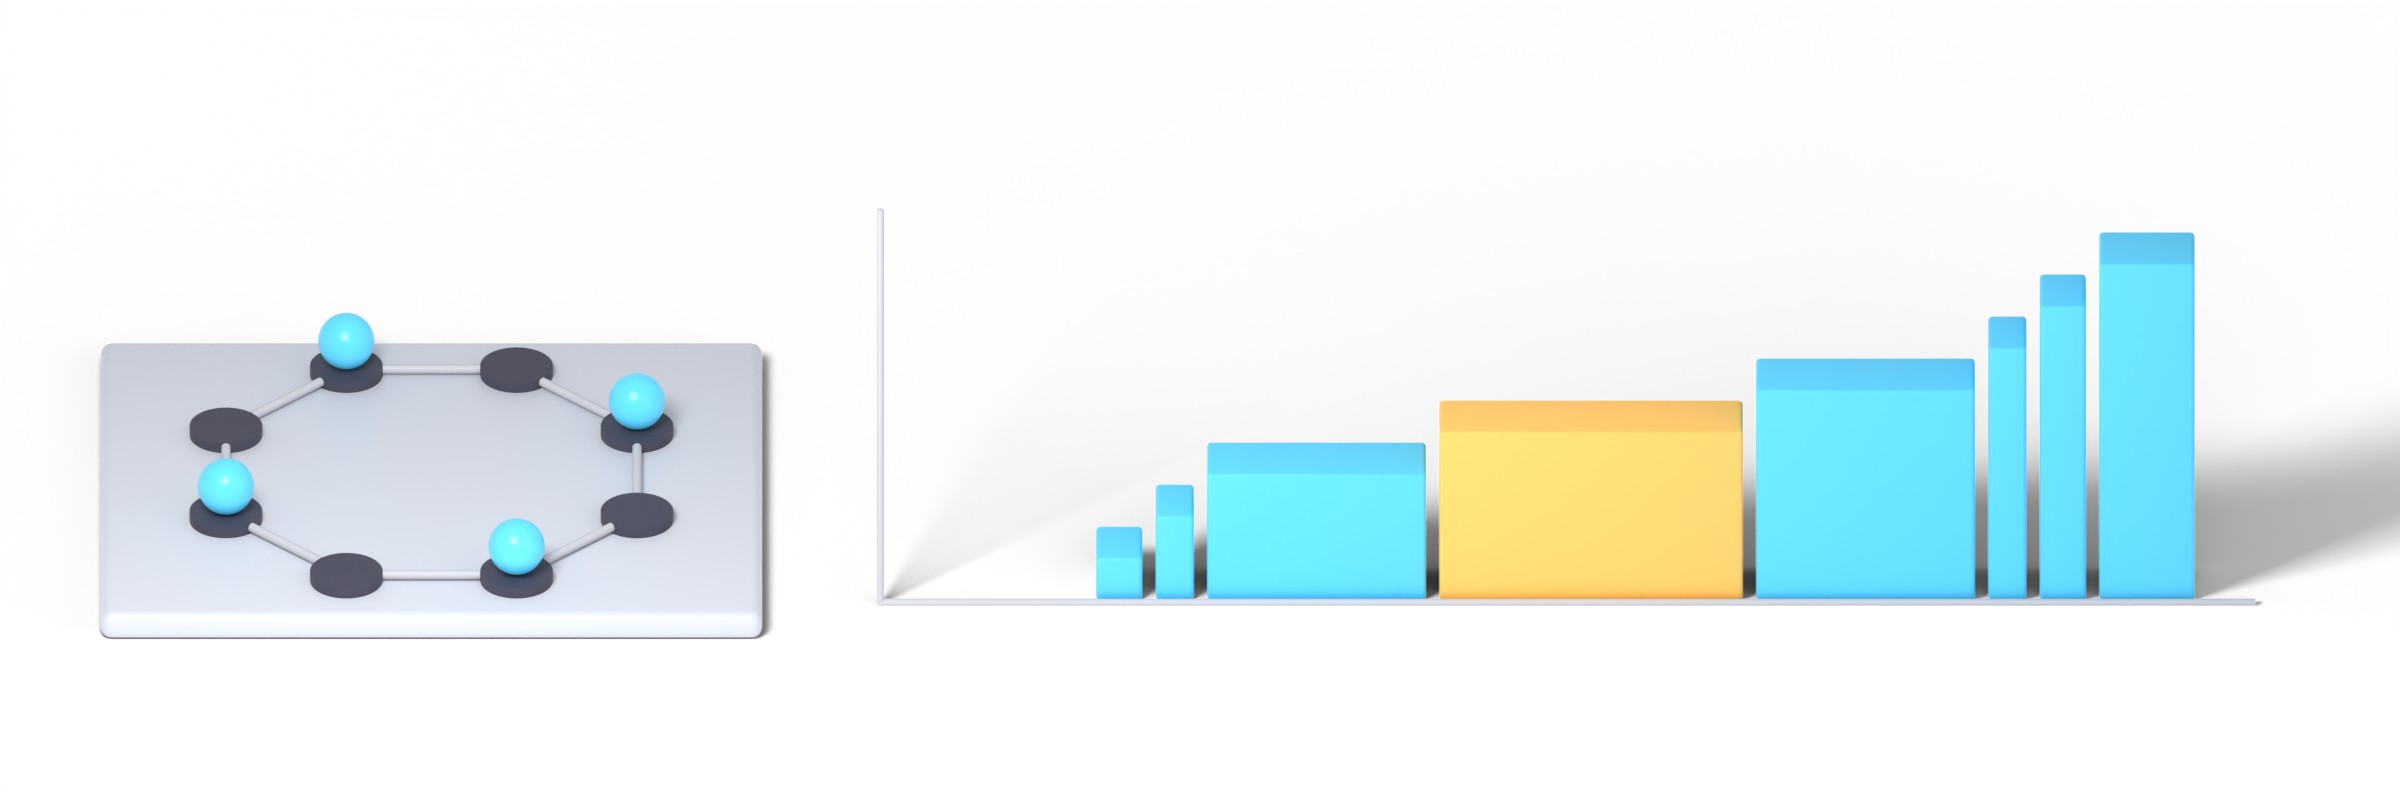
\includegraphics[width=\figw]{../blender/out/charging.jpg}};
  %% written by figlib.py; x and y in units of the image width
\coordinate (a) at (0.0225\figw,0.2577\figw);
\coordinate (gate) at (0.1798\figw,0.0618\figw);
\coordinate (ringN) at (0.1798\figw,0.2118\figw);
\coordinate (muaxis) at (0.9425\figw,0.0825\figw);
\coordinate (Naxis) at (0.3669\figw,0.2459\figw);
\coordinate (gapL) at (0.5969\figw,0.0829\figw);
\coordinate (gapR) at (0.7289\figw,0.0829\figw);
\coordinate (half) at (0.6629\figw,0.1610\figw);
\coordinate (b) at (0.2826\figw,0.2577\figw);
\coordinate (Nzero) at (0.4104\figw,0.0899\figw);
\coordinate (N0) at (0.3669\figw,0.0815\figw);
\coordinate (N4) at (0.3669\figw,0.1516\figw);
\coordinate (N8) at (0.3669\figw,0.2216\figw);

  \node[lbl, font=\normalsize, anchor=west] at (a) {(a)};
  \node[lbl, font=\normalsize, anchor=west] at (b) {(b)};
  \node[lbl, anchor=north] at (gate) {the gate, $-\mu N$};
  \node[lbl, anchor=south] at (ringN) {$N=4$ electrons};
  \node[lbl, anchor=west] at (muaxis) {$\mu$};
  \node[lbl, anchor=south] at (Nzero) {$N=0$};
  \node[lbl, anchor=west] at (Naxis) {$\langle N\rangle$};
  \node[lbl, anchor=east] at (N0) {$0$};
  \node[lbl, anchor=east] at (N4) {$4$};
  \node[lbl, anchor=east] at (N8) {$8$};
  \draw[costamber, <->, thick] ([yshift=-5pt]gapL) -- node[below, font=\small] {charge gap} ([yshift=-5pt]gapR);
\end{tikzpicture}
\end{document}
